% Chapter 1

\chapter{Introduccion} % Main chapter title

\label{Chapter1} % For referencing the chapter elsewhere, use \ref{Chapter1} 

%----------------------------------------------------------------------------------------

% Define some commands to keep the formatting separated from the content 
\newcommand{\keyword}[1]{\textbf{#1}}
\newcommand{\tabhead}[1]{\textbf{#1}}
\newcommand{\code}[1]{\texttt{#1}}
\newcommand{\file}[1]{\texttt{\bfseries#1}}
\newcommand{\option}[1]{\texttt{\itshape#1}}

%----------------------------------------------------------------------------------------

Durante los últimos años, las redes mesh \footnote{Una red mesh es una topología de red local en la que la infraestructura de nodos (routers, Access Points y otros dispositivos) se conectan directamente, dinámicamente y sin jerarquía a tantos otros nodos como sea posible cooperando entre todos para hacer ruteo de la forma más eficiente posible.} han pasado de ser un concepto teórico de red a convertirse en dispositivos comercialmente disponibles que prometen crear redes distribuídas, capaces de crear links entre sí y mantenerlos autónomamente. El IEEE creó el grupo de trabajo 802.11s, que define cómo los dispositivos inalámbricos pueden interconectarse para crear una red  mesh inalámbrica \cite{IEEE802WIKIPEDIA}. Esto tiene la intención de guiar a institutos de investigación y a la industria para desarrollar un estándar para redes mesh, con el objetivo de proveer interoperabilidad entre todos los dispositivos. Mientras el estándar 802.11 sigue bajo desarrollo, hay un número de protocolos de red que están actualmente disponibles.

De todas las aplicaciones de redes mesh, en este trabajo se destacan las redes mesh comunitarias no cableadas, o mesh WCNs (Mesh Wireless Comunity Networks), cuya topología está representada en la figura (\ref{MWCNfigura1}). Estas han sido desarrolladas como movimientos de entusiastas de redes no cabledas, quienes usando equipamiento de bajo costo para una interconexión gratuita, han creado redes completamente autónomas. Su aparición se debe principalmente a la búsqueda de estos grupos de lograr un servicio equivalente a los ofrecidos por redes 2.5G y 3G pero de manera gratuita\cite{PAPERcitadoPORalthea}. 

\begin{figure}[th]	
	\centering	
	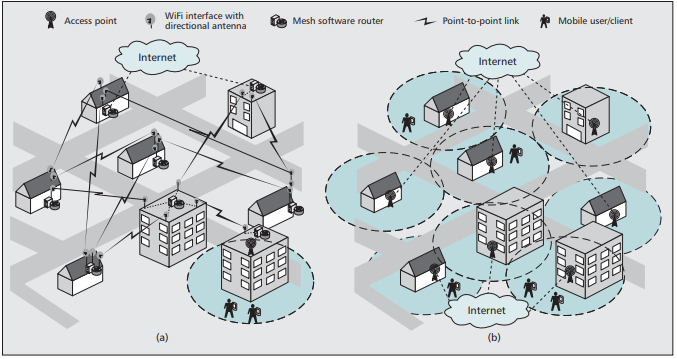
\includegraphics[width=0.95\textwidth]{./figures/WCNs1}		
	\caption{\textit{Topología de redes mesh WCNs. (falta cortar la foto por la mitad y traducirla al castellano)}}
	\label{MWCNfigura1}
\end{figure}



Las razones para participar en una red mesh son muy variadas. Aquellas personas que creen que la conectividad de banda ancha debería ser libre y gratuita y que las barreras impuestas por los oligopolios de los ISPs deben ser eliminadas usualmente son los primeros en unirse a WCNs. En el cuadro (\ref{cuadroWCNS1}), se reportan algunas de las mesh WCNs más significativas a nivel mundial categorizadas según el año en que han sido diseñadas y la cantidad de nodos. Cabe destacar que todas ellas parten de una iniciativa comunitaria, es decir que son el resultado de efuerzos colectivos de voluntarios individuales y funcionan sin fines de lucro.

\begin{table}[th]
\centering
\caption{Comunidades de redes mesh WCNs en todo el mundo.}
\label{cuadroWCNS1}
\begin{tabular}{|c|c|c|c|}
\hline
\textbf{\begin{tabular}[c]{@{}c@{}}Nombre\\   de la Red\end{tabular}} & \textbf{Ubicación}                                                       & \textbf{\begin{tabular}[c]{@{}c@{}}Año de\\   Fundación\end{tabular}} & \textbf{\begin{tabular}[c]{@{}c@{}}Cantidad de\\   nodos\end{tabular}} \\ \hline
SeattleWireless                                                       & \begin{tabular}[c]{@{}c@{}}Seattle, WA, Estados\\   Unidos\end{tabular}  & 2000                                                                  & 80                                                                     \\ \hline
AWMN                                                                  & Athena, Grecia                                                           & 2002                                                                  & 2473                                                                   \\ \hline
CUWiN                                                                 & \begin{tabular}[c]{@{}c@{}}Urbana, IL, Estados\\   Unidos\end{tabular}   & 2002                                                                  & 48                                                                     \\ \hline
\begin{tabular}[c]{@{}c@{}}Berlin's\\   Freifunk\end{tabular}         & Berlin, Alemania                                                         & 2002                                                                  & 316                                                                    \\ \hline
\begin{tabular}[c]{@{}c@{}}Wireless\\   Leiden\end{tabular}           & Leiden, Países Bajos                                                     & 2002                                                                  & 73                                                                     \\ \hline
\begin{tabular}[c]{@{}c@{}}NetEquality\\   Roofnet\end{tabular}       & \begin{tabular}[c]{@{}c@{}}Portland, OR, Estados\\   Unidos\end{tabular} & 2007                                                                  & 126                                                                    \\ \hline
NYCwireless                                                           & \begin{tabular}[c]{@{}c@{}}New York, Estados\\   Unidos\end{tabular}     & 2001                                                                  & 145                                                                    \\ \hline
\end{tabular}
\end{table}

En el estudio de este fenómeno, se destacó la iniciativa de la empresa Althea, con la cual se desarrolló este trabajo en conjunto. Althea propone un modelo de negocios basado en el incentivized mesh \footnote{Explicar con palabras mas bonitas que el incentivized mesh es basicamente pagarle a la gente para que comparta un poquito de su ancho de banda.}. Y aca explicar un poquito brevemente qué hace althea (basicamente copipastear la primera parte de su white paper sin entrar en detalles tecnicos de que tipos de nodos tienen, etc.).

En este parrafo explicar un poco la problematica y el hecho de que me di cuenta (hablar siempre en voz pasiva xq sino me agarra toc) que podría integrar las plataformas althea con libremesh (y explicar qué es libremesh usando el pie de página, no hace falta mas en esta instancia ya que lo explicare por completo en la seccion del marco teorico).

En este parrafo explicar brevemente (pero no tan breve como en el resumen) todo lo que hice en el trabajo y las cosas que quedan como propuesta para seguir trabajando en el futuro.

Y en este parrafo poner -en la seccion 1- se vera tal cosa. En el -capitulo 2- tal otra cosa y listo. Es una manera util de ocupar espacio (mas de la mitad de los papers que lei lo hacen asi que yo tambien lo hare). 
